
\section{Supervised Kick Learning}

\begin{figure}[H]
    \centering
    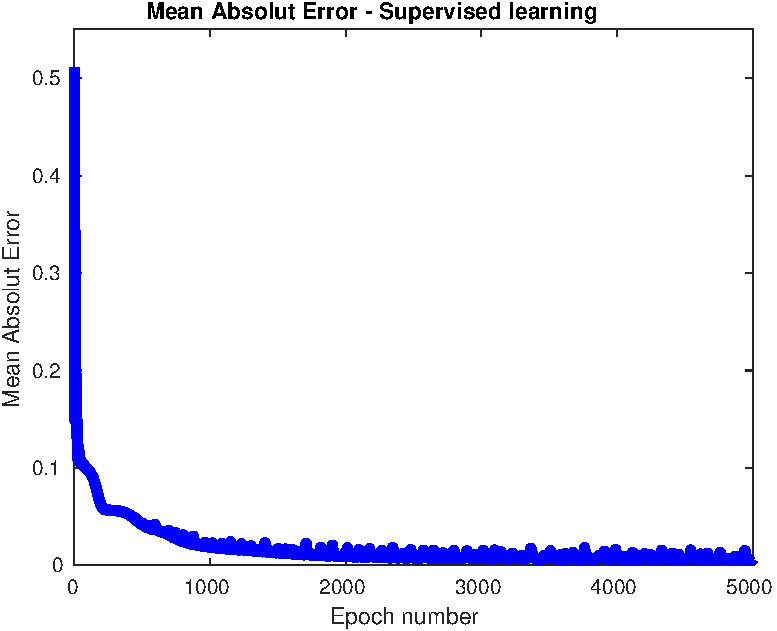
\includegraphics[width=0.6\textwidth]{Chapter7/plots/plot_MAE_supervised.pdf} 
    \caption{Mean Absolut Error - SL.}
    \label{fig:SL_MAE}
\end{figure}

\begin{figure}[H]
    \centering
    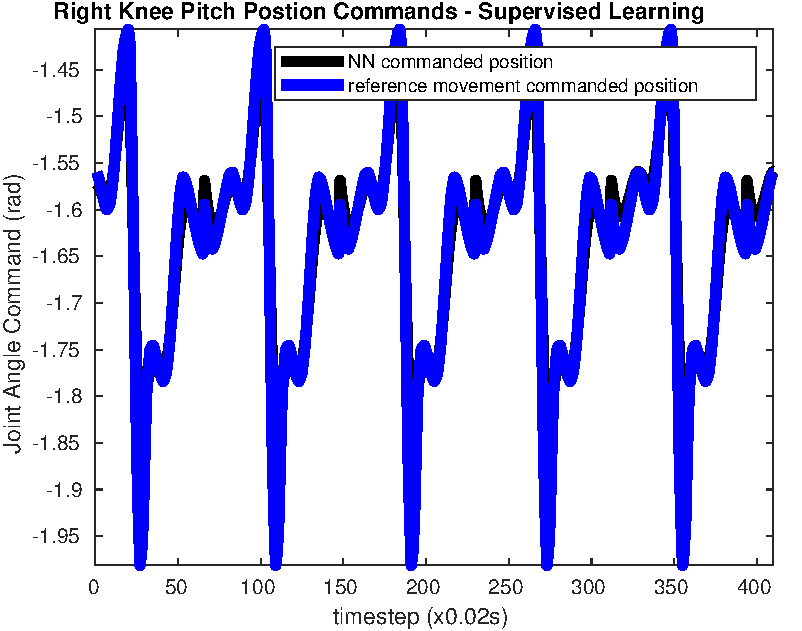
\includegraphics[width=0.6\textwidth]{Chapter7/plots/plot_joints_pos_superv.pdf} 
    \caption{Commanded Position for the Right Knee Pitch Joint - SL.}
    \label{fig:SL_cmd_pos}
\end{figure}

\section{Pure Mimic Learning}

\begin{figure}[H]
    \centering
    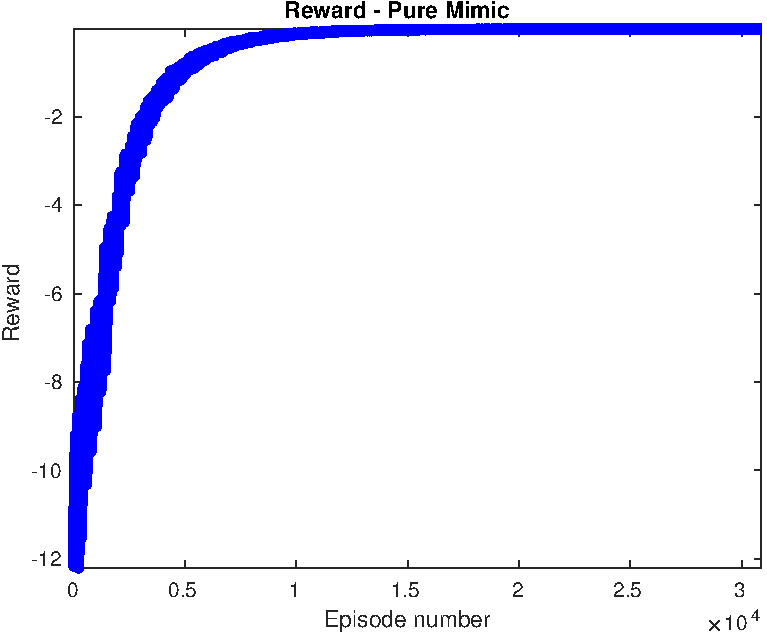
\includegraphics[width=0.6\textwidth]{Chapter7/plots/plot_reward_mimic.pdf} 
    \caption{Reward signal during training for the mimic task.}
    \label{fig:RL_mimic_reward}
\end{figure}

\begin{figure}[H]
    \centering
    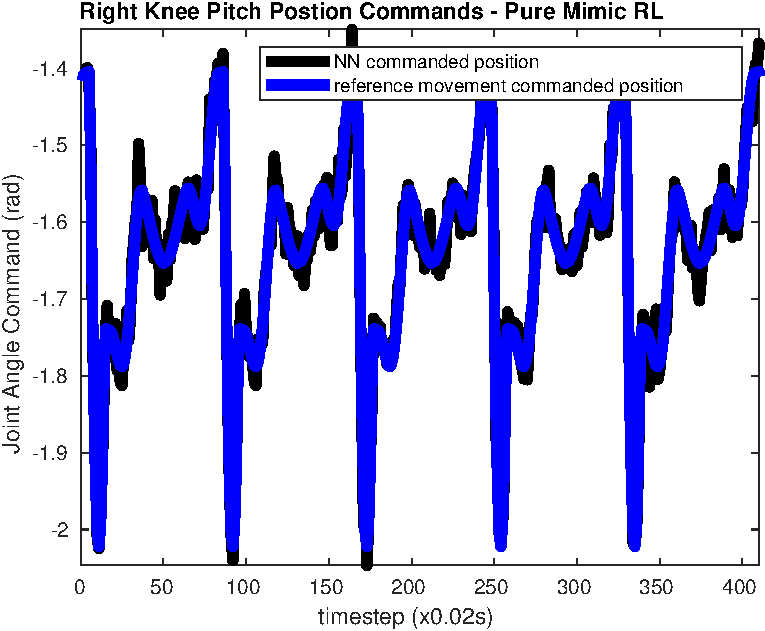
\includegraphics[width=0.6\textwidth]{Chapter7/plots/plot_joints_pos_mimic.pdf} 
    \caption{Commanded Position for the Right Knee Pitch Joint - mimic RL.}
    \label{fig:RL_cmd_pos}
\end{figure}

\section{Farthest Final Distance Learning}

\begin{figure}[H]
    \centering
    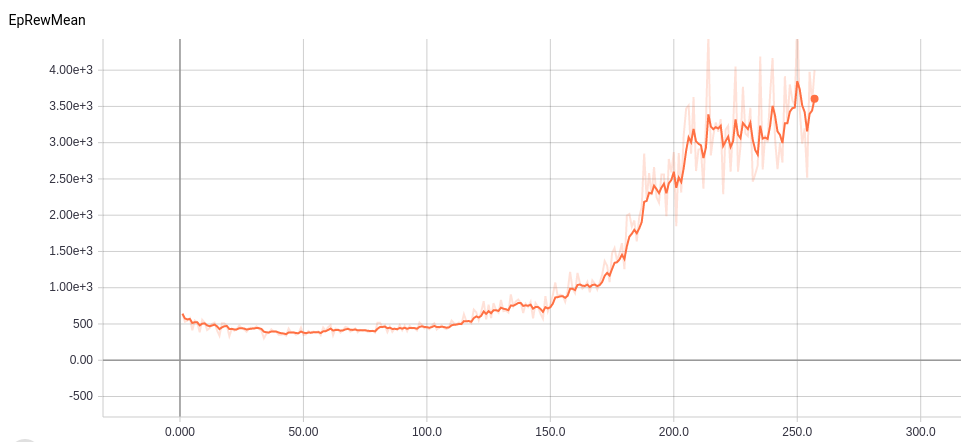
\includegraphics[width=0.8\textwidth]{Chapter7/figures/rew_mean_far_kick.png} 
    \caption{Reward signal during training for the farthest kick task.}
    \label{fig:RL_far_kick}
\end{figure}

\begin{figure}[H]
    \centering
    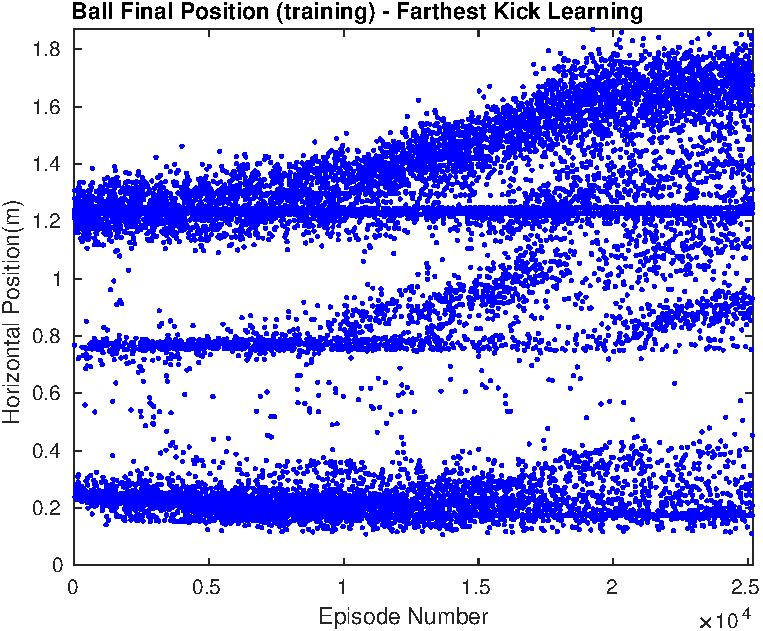
\includegraphics[width=0.6\textwidth]{Chapter7/plots/plot_ball_pos_far_kick_train.pdf} 
    \caption{Ball final positions during training - farthest kick task.}
    \label{fig:RL_far_kick_pos_train}
\end{figure}

\begin{figure}[H]
    \centering
    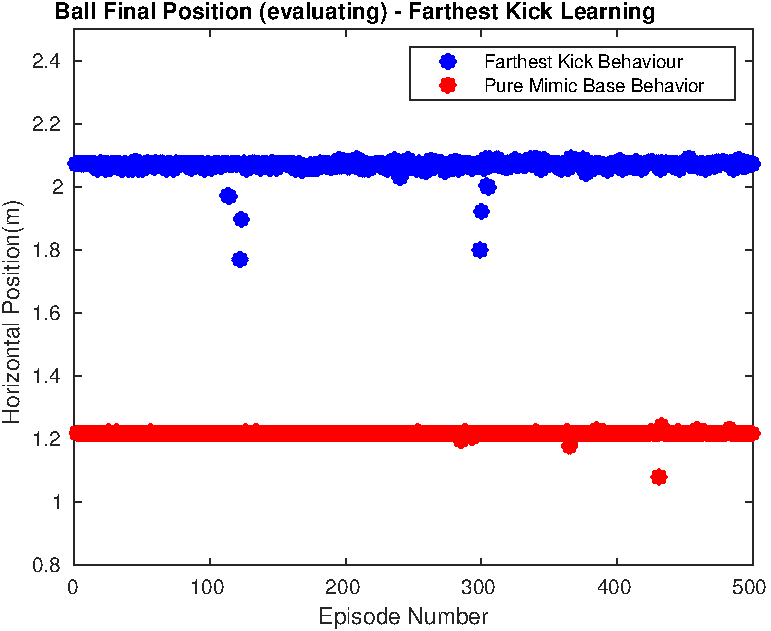
\includegraphics[width=0.6\textwidth]{Chapter7/plots/plot_ball_pos_far_kick_eval.pdf} 
    \caption{Ball final positions during evaluation - farthest kick task.}
    \label{fig:RL_far_kick_pos_eval}
\end{figure}

\begin{figure}[H]
    \centering
    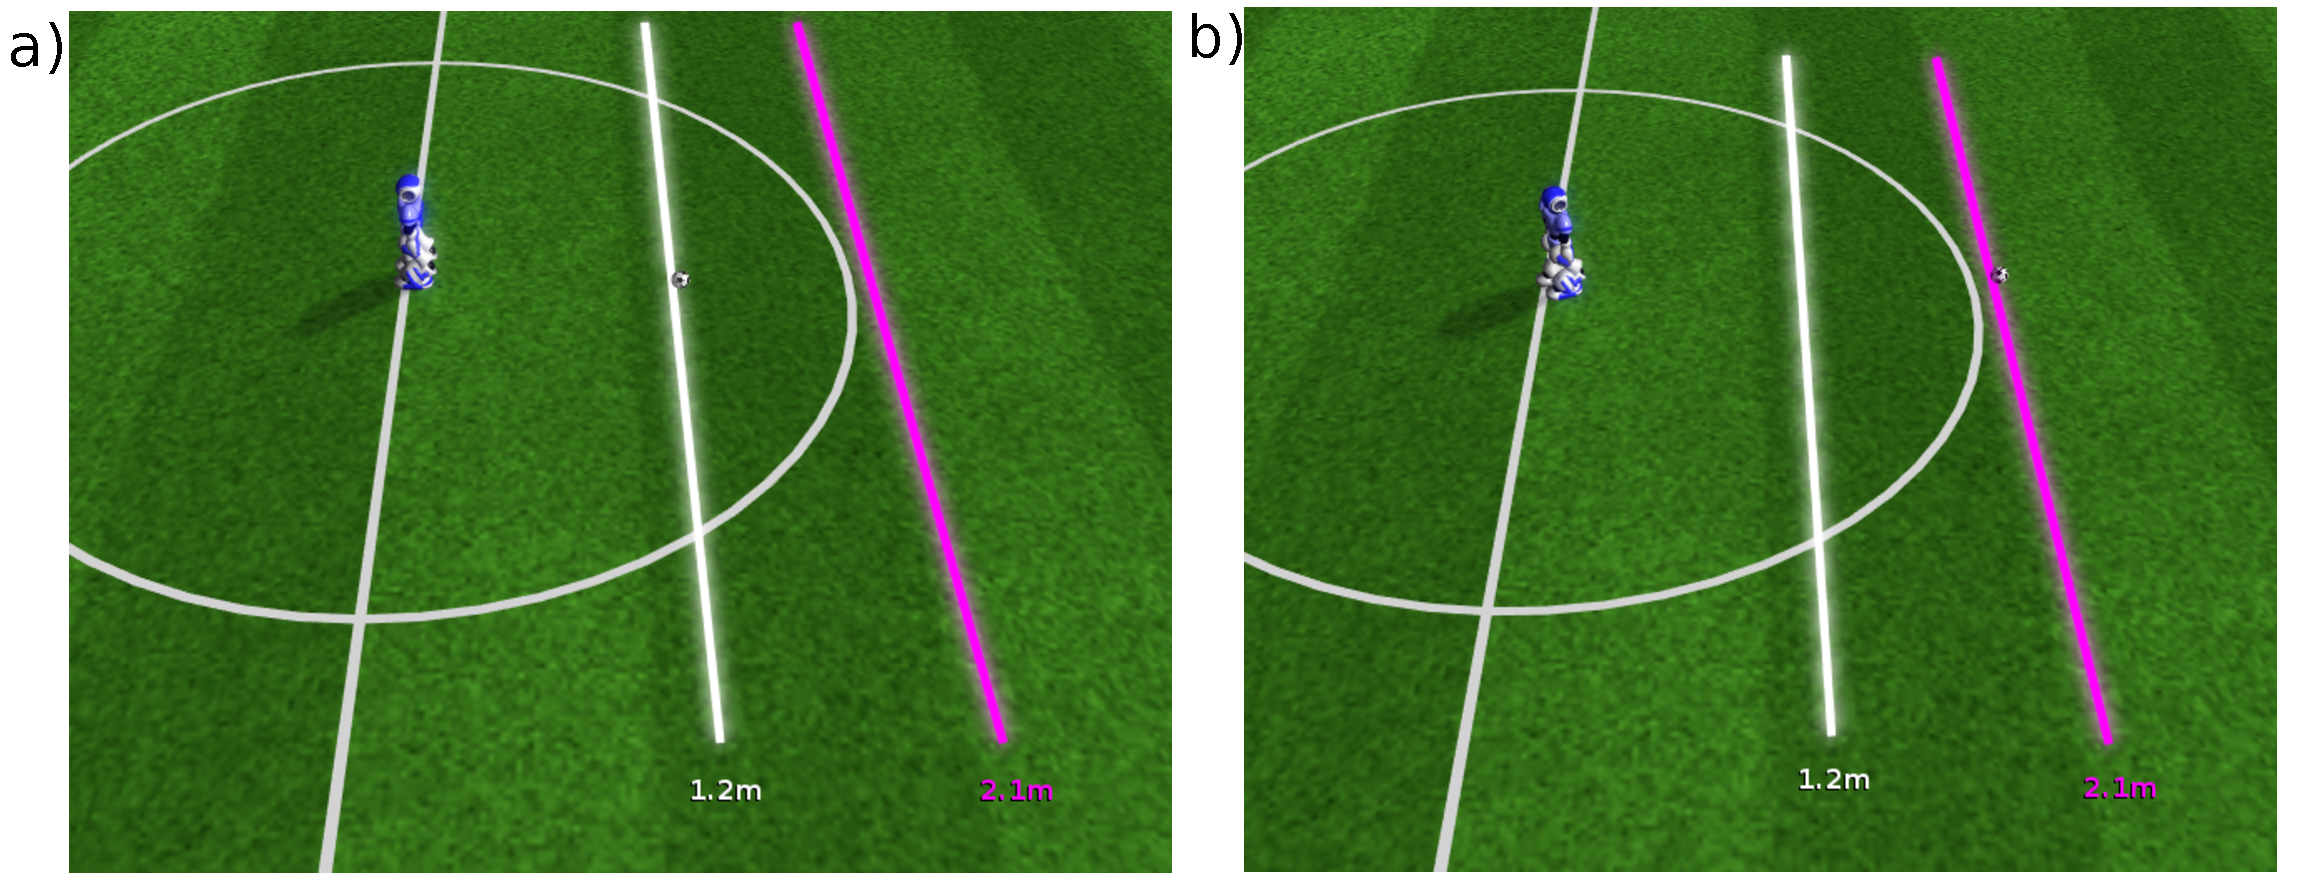
\includegraphics[width=1.0\textwidth]{Chapter7/figures/kick_far.pdf} 
    \caption{Game play illustration. a)Reference final position. b)Learned behavior final position}
    \label{fig:RL_far_kick_roboviz}
\end{figure}

\section{Fixed Final Distance Learning}

\subsection{0.8m Fixed Distance}

\begin{figure}[H]
    \centering
    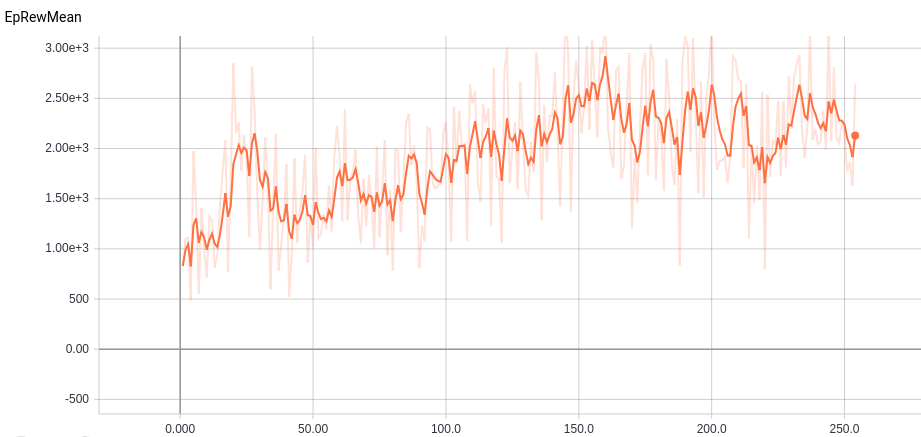
\includegraphics[width=0.8\textwidth]{Chapter7/figures/rew_mean_fix_08.png} 
    \caption{Reward signal during training for the fixed 0.8 distance task.}
    \label{fig:RL_08_kick}
\end{figure}

\begin{figure}[H]
    \centering
    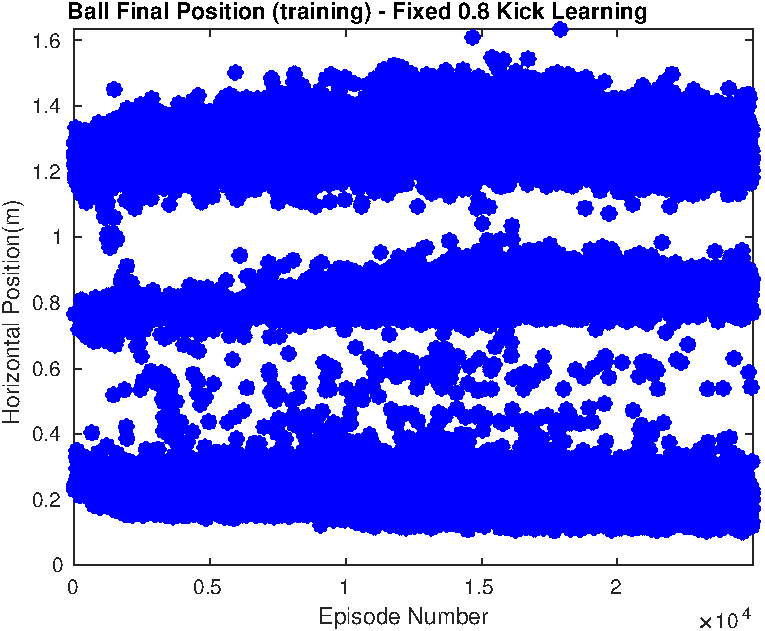
\includegraphics[width=0.6\textwidth]{Chapter7/plots/plot_ball_pos_08fix_kick_train.pdf} 
    \caption{Ball final positions during training - fixed 0.8 distance task.}
    \label{fig:RL_08_kick_pos_train}
\end{figure}

\begin{figure}[H]
    \centering
    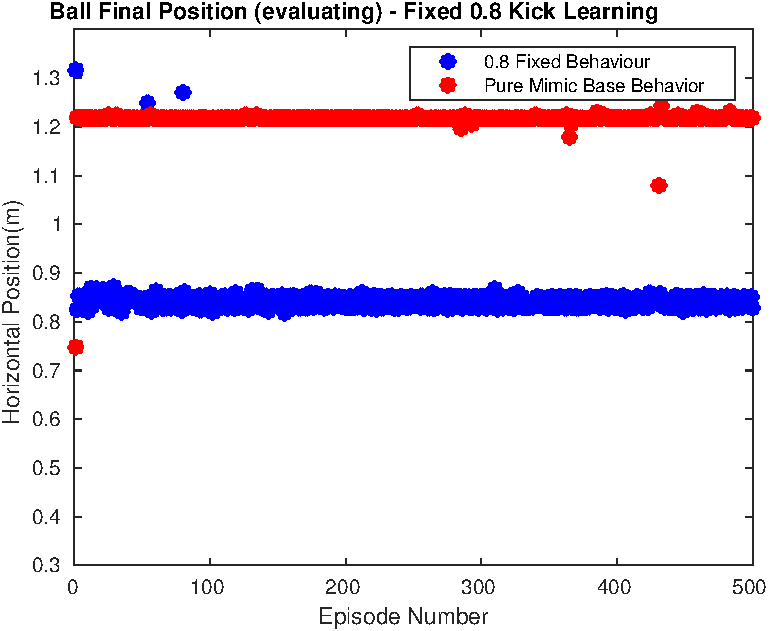
\includegraphics[width=0.6\textwidth]{Chapter7/plots/plot_ball_pos_08fix_kick_eval.pdf} 
    \caption{Ball final positions during evaluation - fixed 0.8 distance task.}
    \label{fig:RL_08_kick_pos_eval}
\end{figure}

\begin{figure}[H]
    \centering
    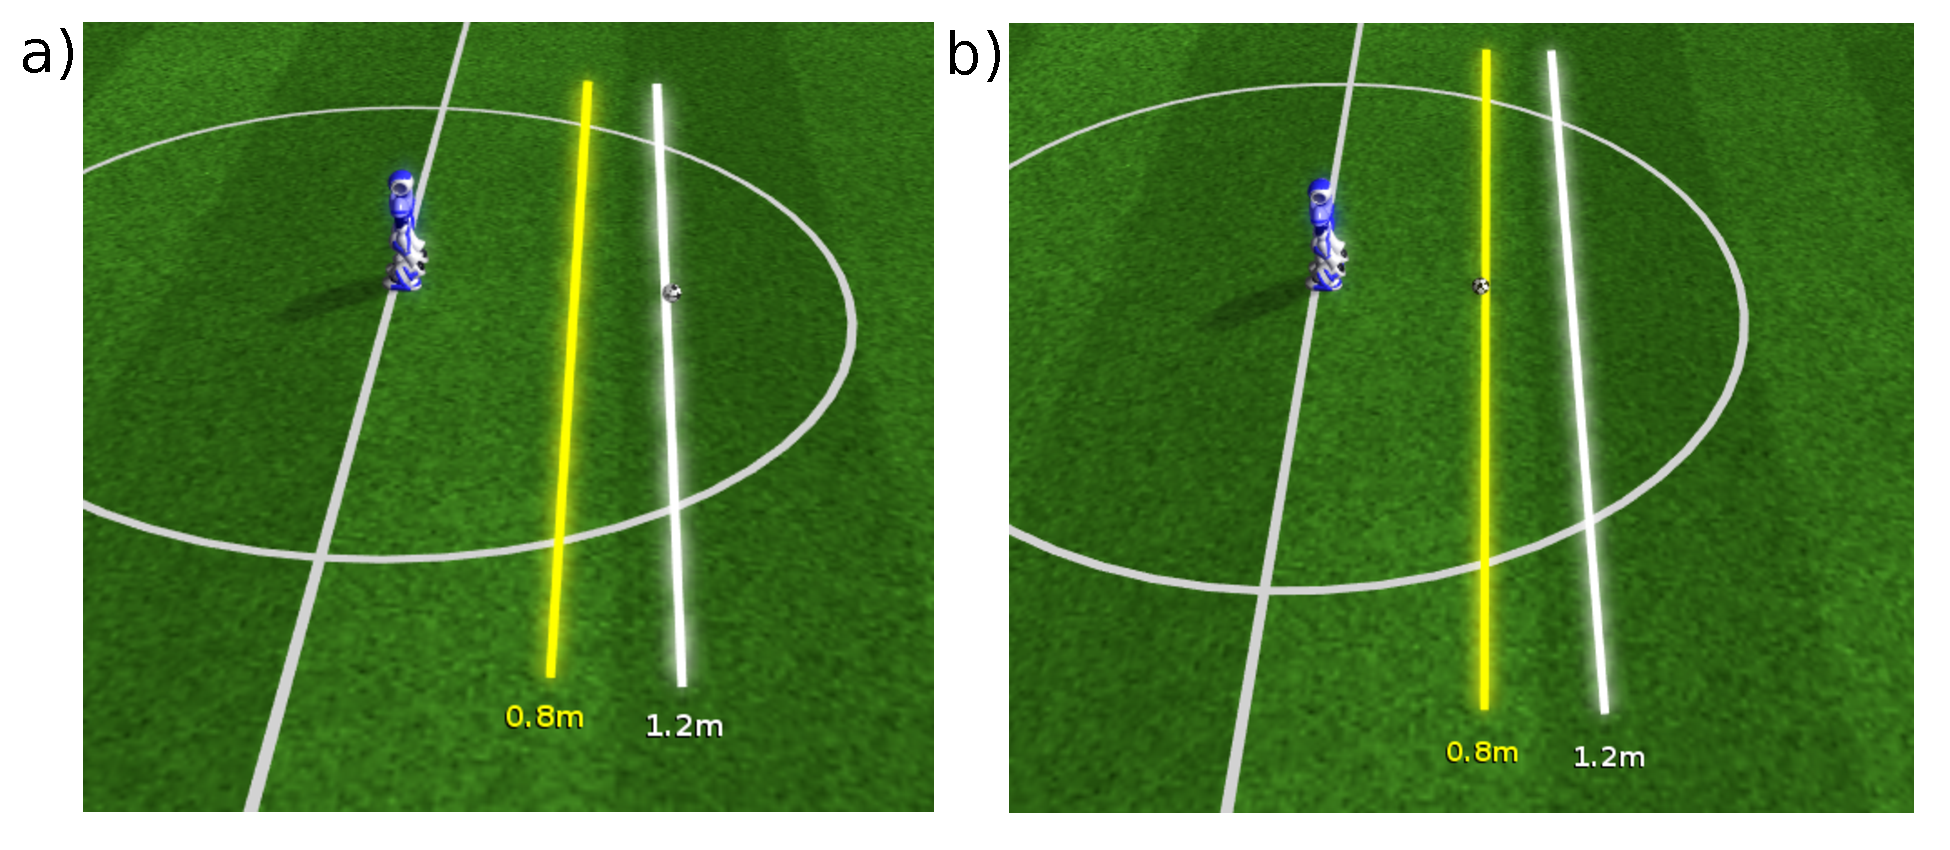
\includegraphics[width=1.0\textwidth]{Chapter7/figures/kick_train_08.pdf} 
    \caption{Game play illustration. a)Reference final position. b)Learned behavior final position}
    \label{fig:RL_08_kick_roboviz}
\end{figure}

\subsection{1.5m Fixed Distance}

\begin{figure}[H]
    \centering
    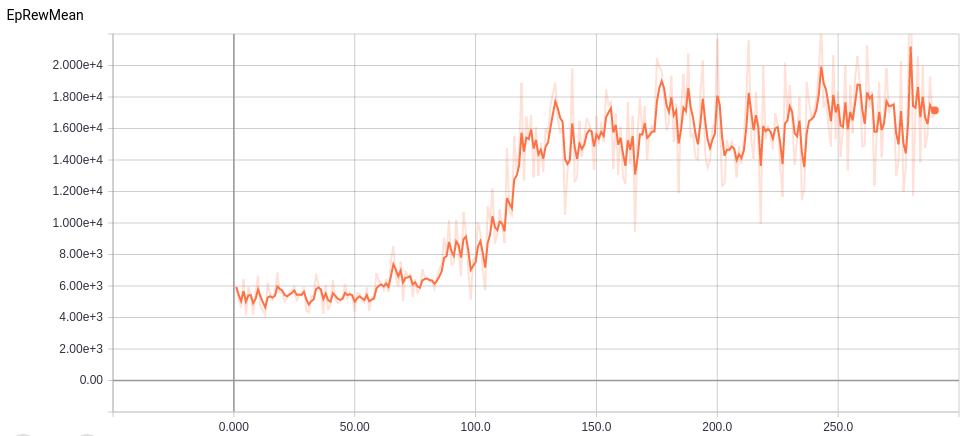
\includegraphics[width=0.8\textwidth]{Chapter7/figures/rew_mean_fix_15.png} 
    \caption{Reward signal during training for the fixed 1.5 distance task.}
    \label{fig:RL_15_kick}
\end{figure}

\begin{figure}[H]
    \centering
    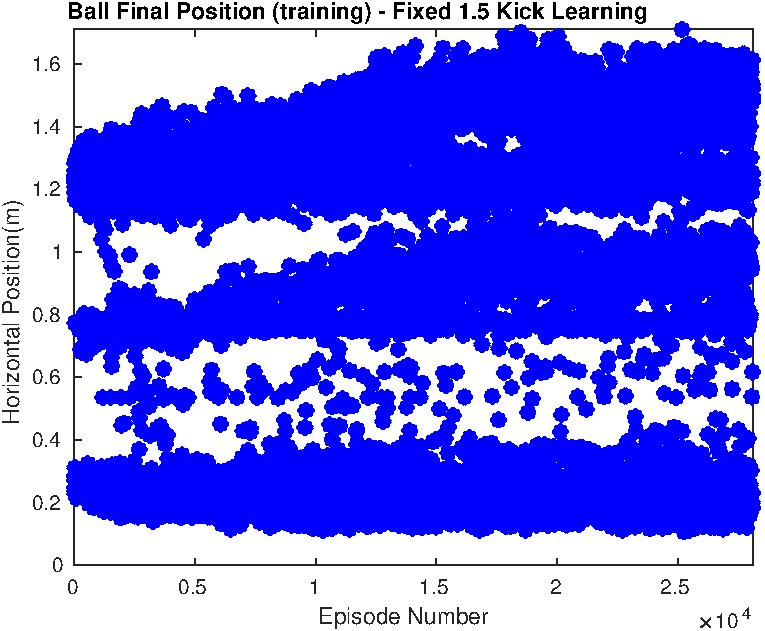
\includegraphics[width=0.6\textwidth]{Chapter7/plots/plot_ball_pos_15fix_kick_train.pdf} 
    \caption{Ball final positions during training - fixed 1.5 distance task.}
    \label{fig:RL_15_kick_pos_train}
\end{figure}

\begin{figure}[H]
    \centering
    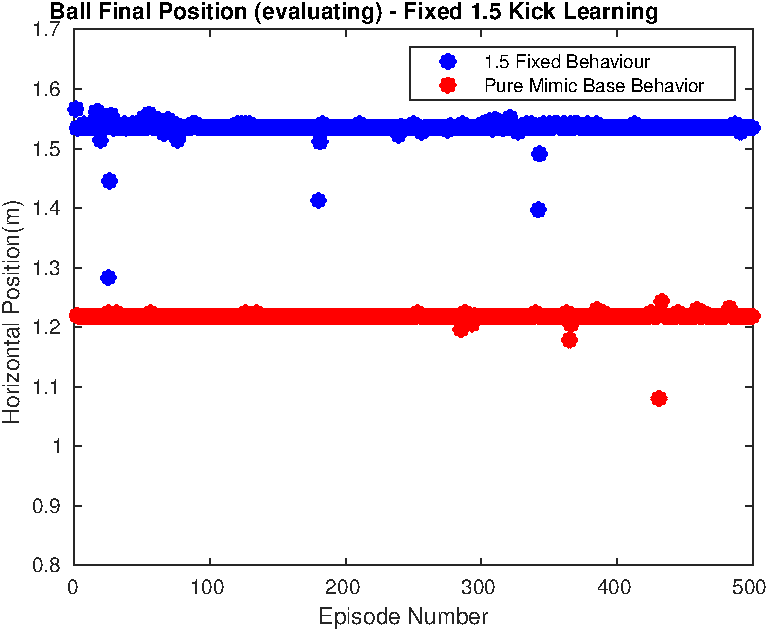
\includegraphics[width=0.6\textwidth]{Chapter7/plots/plot_ball_pos_15fix_kick_eval.pdf} 
    \caption{Ball final positions during evaluation - fixed 1.5 distance task.}
    \label{fig:RL_15_kick_pos_eval}
\end{figure}

\begin{figure}[H]
    \centering
    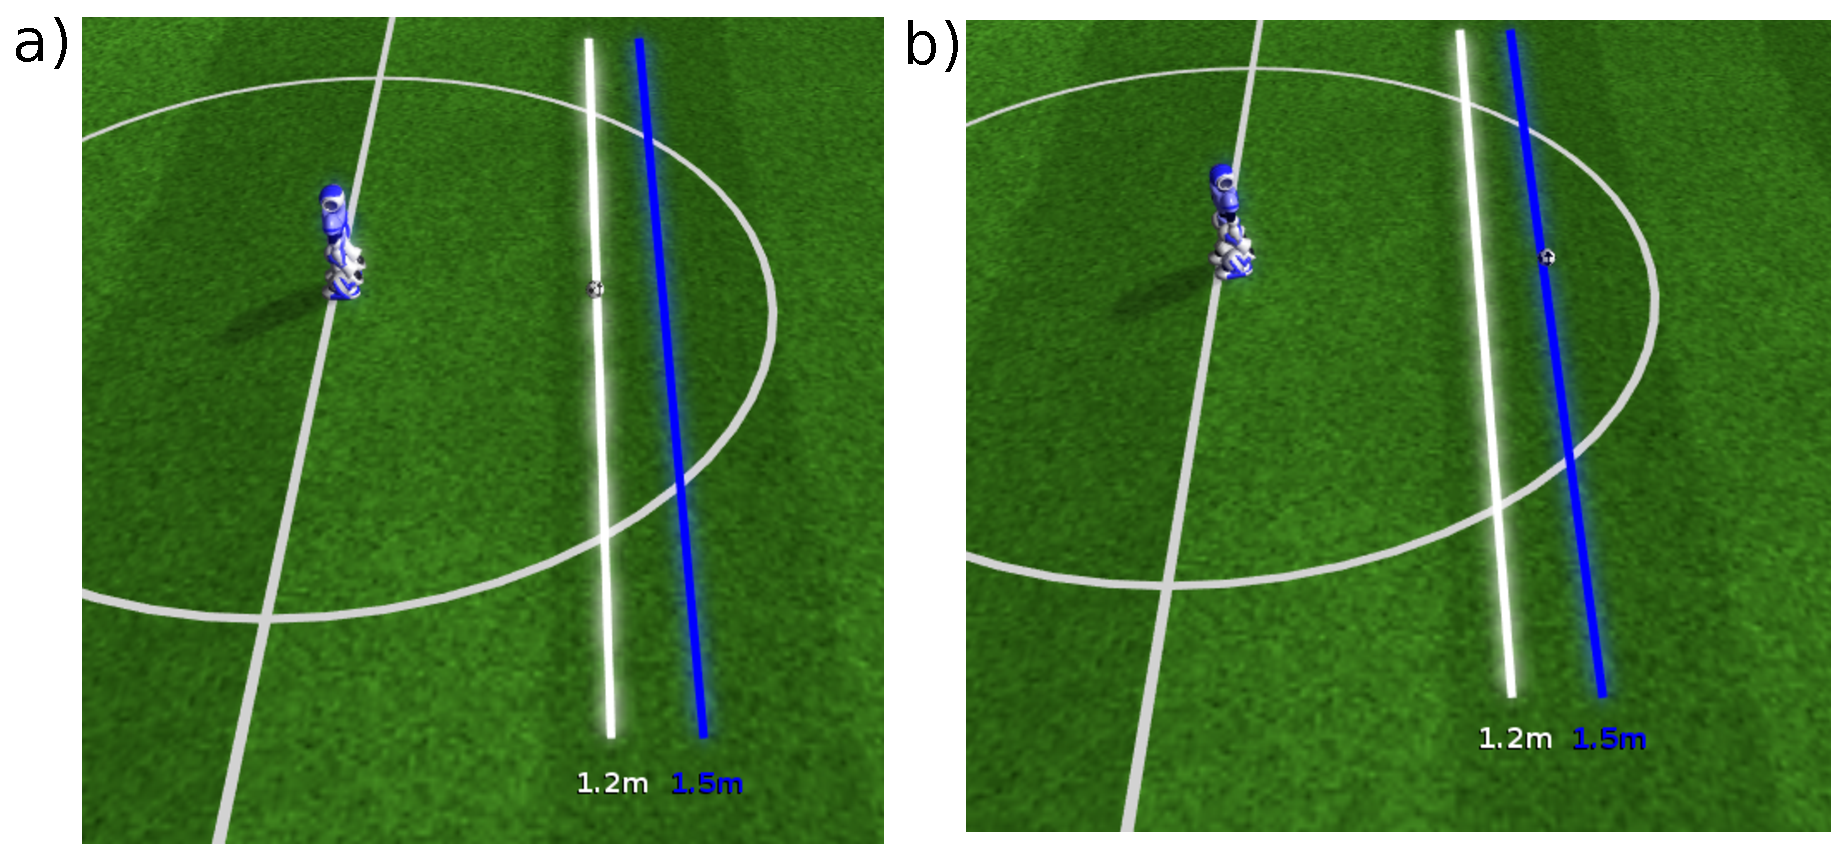
\includegraphics[width=1.0\textwidth]{Chapter7/figures/kick_train_15.pdf} 
    \caption{Game play illustration. a)Reference final position. b)Learned behavior final position}
    \label{fig:RL_15_kick_roboviz}
\end{figure}